\documentclass{amsart} 
\usepackage{graphicx}
\graphicspath{{./}}
\usepackage[fontsize=14pt]{scrextend}
\usepackage{hyperref}
\usepackage{csvsimple}
\usepackage{epigraph}
\title{Single Motherhood is lowest in Middle East and North Africa but that does not imply Islam solves the problem}
\author{Zulfikar Moinuddin Ahmed}
\date{\today}
\begin{document}
\maketitle

\section{Reminder that I am not Muslim}
Yes, my name is classical Arabic Muslim name.  And I am not Muslim. I've been Atheist since six and have my own values and faith that is not Islam.  My values are closer to West than Islam, and closer to Europe than America by measurements.  I am not Muslim, definitely not Muslim.  I don't think Muslims are bad people, but I am not Muslim, thank you very much.

\section{Single Motherhood levels by Continents}

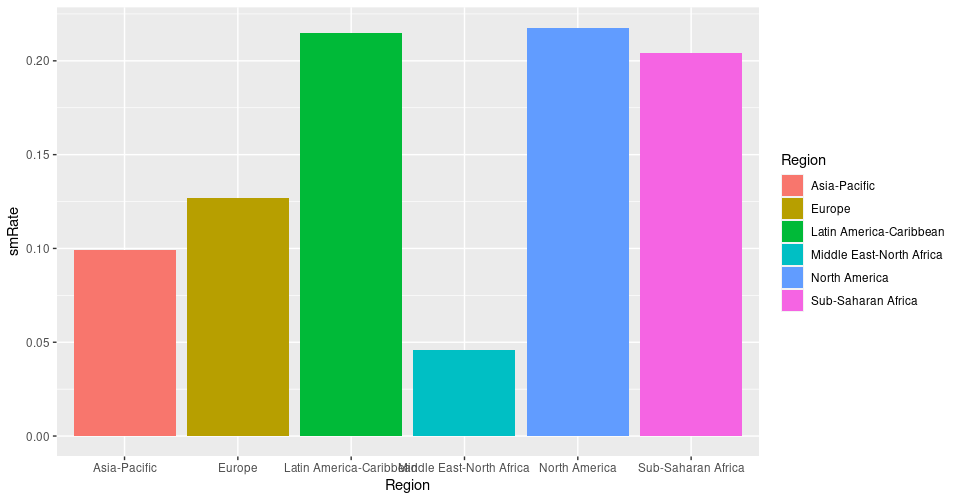
\includegraphics[scale=0.45]{smc.png}

The data are from \cite{PR} and the graph was done with dplyr manipulations in R.  The most striking feature is that North Africa and Middle East, Muslim countries have a phenomenally low single mother rate.  Europe is quite low as well after Asia.  

A natural response might be that Islam provides the resolution of the problem, and that answer is totally wrong.  Unless a group gave zero answer, I am unlikely to consider the religion as the major factor.  This is because these are universal issues.  Islam falls under 'traditional-survivalist' values in the World Value Survey, and that affects this problem mostly because fatherhood in Islam and in East and Southeast Asia are still unchallenged.  Now I believe fatherhood is under severe pressure in the west.  


\begin{thebibliography}{CCC}
\bibitem{PR}{\url{https://www.pewforum.org/wp-content/uploads/sites/7/2019/12/
PF_12.12.19_religious.households_data.xlsx}}
\end{thebibliography}
\end{document}
